\begin{figure}[H]
\centering
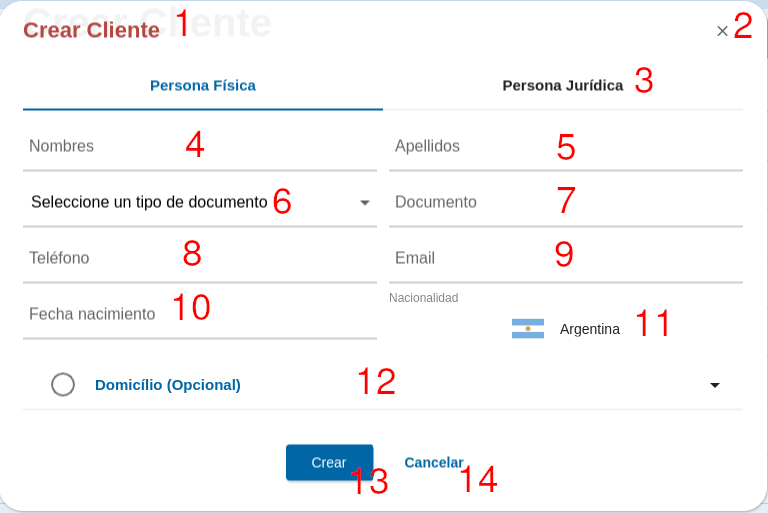
\includegraphics[width=\textwidth,height=\textheight,keepaspectratio]{Escenarios/AD-29-00}
\caption{Escenario - AD-29-00}
\label{fig:AD-29-00}
\end{figure}
Este escenario permite a los usuarios crear o modificar clientes. El campo \textbf{AD-29-01} indica la operación que se esta realizando, pudiendo ser 'Crear cliente' o 'Editar cliente'.
Con el botón \textbf{AD-29-02} se podrá cerrar la ventana y volver al escenario \textbf{AD-28-00}.
En el caso que la operación sea 'Editar', los campos: \textbf{AD-29-04}, \textbf{AD-29-05}, \textbf{AD-29-06}, \textbf{AD-29-07}, \textbf{AD-29-08}, \textbf{AD-29-09}, \textbf{AD-29-10}, y \textbf{AD-29-11} estarán autocompletados con los datos del cliente a editar.
El botón \textbf{AD-29-03} permite indicar que se está creando o modificando un cliente que es una persona jurídica, en dicho caso los campos \textbf{AD-29-04} y \textbf{AD-29-05} se reemplazan por un único para indicar la razón social. El cliente debe completar el formulario para crear o editar un cliente, indicando en el campo \textbf{AD-29-04} los nombres, en el campo \textbf{AD-29-05} los apellidos, seleccionado de la lista desplegable \textbf{AD-29-06} el tipo de documento, especifando el número de documento en el campo \textbf{AD-29-07}, el número de teléfono en el campo \textbf{AD-29-08}, el correo electrónico en el campo \textbf{AD-29-09}, fecha de nacimiento en el campo \textbf{AD-29-10} y seleccionado la nacionalidad en de la lista desplegabale \textbf{AD-29-11}. 
Un click en el botón \textbf{AD-29-12} desplegara un formulario para que el usuario complete con los datos del domicilio del cliente.
Un click en el botón \textbf{AD-29-13} creará o modificará al cliente según corresponda y navegará al escenario \textbf{AD-28-00}, mientras que click en el botón \textbf{AD-29-14} cerrará la ventana y navegará al escenario \textbf{AD-28-00}.
\clearpage
